%% -*- coding:utf-8 -*-
\begin{figure}
\centering
\ifpdf
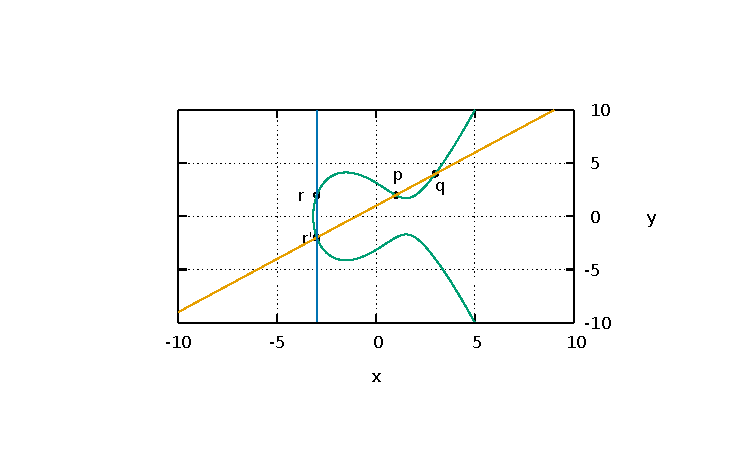
\includegraphics[angle=0,scale=1.5]
{./add/discretmath/picellipticsum.pdf}
\else
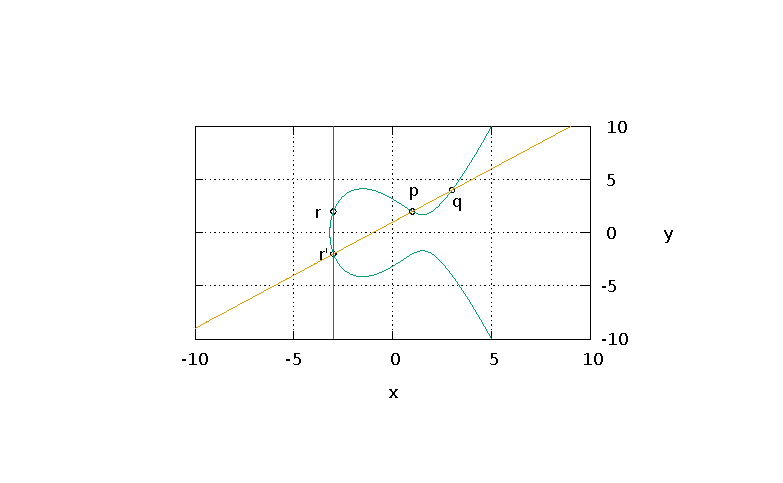
\includegraphics[angle=0,scale=1.5]
{./add/discretmath/picellipticsum.eps}
\fi
\caption{Elliptic curve $y^2 = x^3 -7 x + 10$ over the field of
  real numbers $\mathbb{R}$. Addition of two points $p(1,2)$ and
  $q(3,4)$. The line passing through these points intersects the curve at
  a third point $r'(-3,-2)$. The point $r(-3,2)$ symmetric to $r'$
  with respect to the curve is the sum of the original two: $p + q = r$}
\label{fig:add:ellipticRsum}
\end{figure}